
\documentclass[]{article}

\title{Universidad Autónoma de Nuevo León
Facultad de Ingeniería Mecánica}

\date{}
\usepackage{braket}
\usepackage{bbold}
\usepackage{amsmath,amsfonts,amssymb,amsthm}
\usepackage[margin=1.0in]{geometry}
\usepackage{graphicx}
\usepackage{chngcntr}

\usepackage[backend=biber]{biblatex}
\addbibresource{ref.bib}
\begin{document}
	\maketitle
	\begin{center}


\centerline{\textbf{TAREA 1:} } 
\textbf{MODELOS PROBABILISTAS APLICADOS. 
ANÁLISIS DE VISITANTES INTERNACIONALES 
QUE INGRESARON AL PAÍS EN EL 2020}
\linebreak
\linebreak
\linebreak
\linebreak
\linebreak
\linebreak
\centerline{Profesor: } 
\centerline{DRA. SATU ELISA SCHAEFFER}
\linebreak
\linebreak
\linebreak
\centerline{Alumno: } 
\centerline{Joaquín Arturo Velarde Moreno}
\linebreak
\linebreak
\linebreak
\centerline{Matería: } 
\centerline{MODELOS PROBABILISTAS APLICADOS}
	\end{center}
	
		\cite{inegi}
		
		
\newpage

\section*{Origen de los datos:}
Los datos que a continuación se analizarán fueron publicados por el INEGI\cite{inegi} en el apartado de Turismo y se obtuvieron mediante la aplicación de una serie de encuestas a viajeros que arribaron del extranjero a México durante el periodo de agosto del 2018 a junio del 2020. Dichos datos se publicaron en formatos XLSX.

\section*{Metodología:}
Esta sección de datos se concentró, generó y editó en Microsoft Excel\cite{excel} proveyendo información preliminar de los meses enero, febrero, marzo, abril, mayo y junio.\\

Además. se creó un diagrama de cajas y bigotes que representa de manera visual el conjunto de visitantes por mes, obteniendo los siguientes datos: mínimo, máximo, media, primer cuartil y tercer cuartil. Los cuales fueron analizados utilizando el programa R versión 4.0.2\cite{rproject}.\\

En la figura \ref{fig:mesh} se puede observar la clasificación del tipo de turistas categorizándose en cuatro apartados:
\begin{enumerate}
	\item turistas de internación
	\item  turistas fronterizos 
	\item excursionistas fronterizos
	\item excursionistas en cruceros.
\end{enumerate}
\subsection*{Turistas de internación:}
Los turistas de internación son los que se adentran en el territorio nacional por vía aérea y terrestre, aunque la mayoría, como se puede observar, prefieren la internación aérea.
\subsection*{Turistas fronterizos:}
Los turistas fronterizos son aquellos que viajan a las ciudades fronterizas de nuestro país desplazándose ya sea mediante automóvil o de manera peatonal.
\subsection*{Excursionistas fronterizos:}
Los excursionistas fronterizos cruzan principalmente la frontera para hacer compras y retornan sin quedarse en el territorio nacional, ya sea en automóvil o de forma peatonal. 
\subsection*{Excursionistas de crucero:}
Los excursionistas de crucero son pasajeros que visitan un puerto mexicano sin quedarse la noche en México; es decir, llegan al puerto, conocer, hacen compras y regresan al crucero. Resalta en este apartado que, debido a la crisis sanitaria por la pandemia del COVID-19, en los últimos meses, el número de excursionistas de crucero ha sido de 0.
		
\newpage
\subsection*{Gráfico:}
	\counterwithin{figure}{section}
	\begin{figure}[h]
    	\centering
    	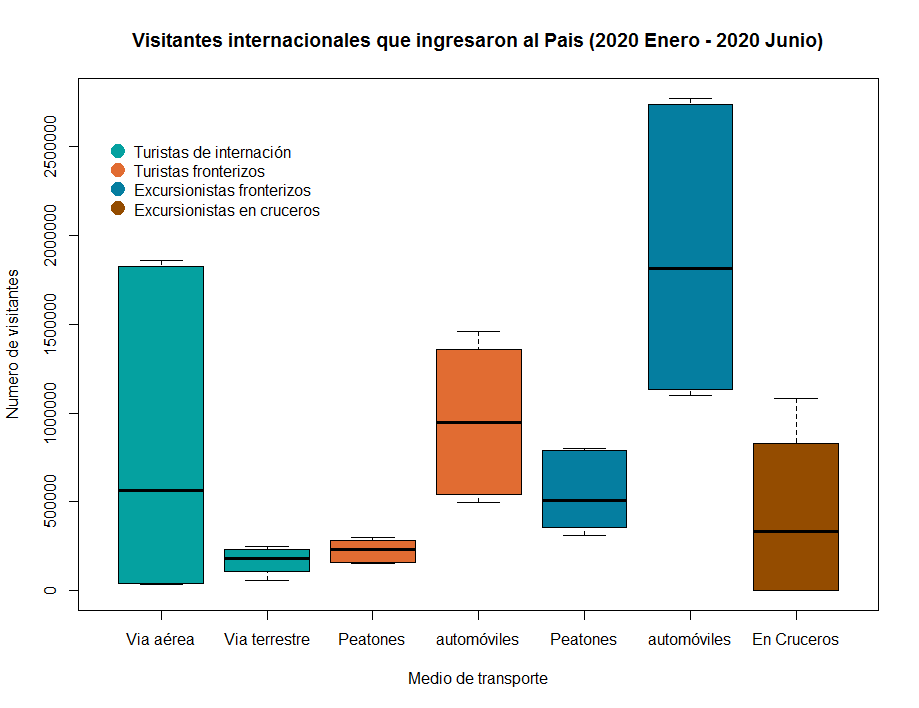
\includegraphics[scale=.5]{Turismo}
    	\caption{Visitantes internacionales por tipo}
    	\label{fig:mesh}
	\end{figure}

\printbibliography[title={Referencias}]
\end{document}
